%%%%%%%%%%%%%%%%%%%%%%%%%%%%%%%%%%%%%%%%%%%%%%%%%%%%%%%%%%%%%%%%%%%%%%%%%%%%%%%%
\section{Experiments}
\label{sec:experiment}

\subsection{Experimental Configuration}
\label{sec:method_terrain}

\subsubsection{Simulation Environment} All policies are trained using NVIDIA Isaac Gym~\cite{Isaac_Gym} on an NVIDIA RTX 4090 GPU with a 12-DoF Unitree G1 humanoid robot. LiDAR point clouds are synthesized using the simulator from~\cite{Wang_2025_Omni-Perception}, which can accurately model sensor noises and occlusion from static terrains and dynamic robot links.

\subsubsection{Real-world Environment} The trained policy is then deployed on a physical Unitree G1 robot. A Livox Mid-360 LiDAR is mounted on the head to provide raw point cloud data. State estimation and point cloud registration are handled by Fast-LIO2~\cite{Xu_2022_FAST-LIO2}. Both the horizontal and vertical elevation maps $\mathbf{E}_t$ are extracted from the registered point cloud using the GPU-accelerated pipeline from~\cite{ElevationMap_GPU_2022} at $10$ Hz. 
% The vertical distance map $\mathbf{D}_t$ is generated at $10$ Hz as well. Registered points are projected into a polar sector spanning $-45^\circ$ to $+45^\circ$. Each map cell records the distance to the nearest obstacle. 
The map generation follows the exact same procedure used in simulation. Joint commands are executed at $50$ Hz on an onboard NVIDIA Jetson Orin NX.

\subsection{Simulation Experiments}
\subsubsection{Evaluation Setup}
All methods are evaluated on the highest difficulty tier of \textit{BarrierTrack}. The benchmark includes all seven terrain primitives, grouped into two categories: terrains that require precise foot placement like Stairs, Drop, Jump and Hurdle, and the others that require traversable-space selection like Beam, Pole and Narrow Gate. For each terrain type, every episode contains five obstacles of the same class with progressively increasing difficulty; obstacle parameters are sampled within the range given in Table~\ref{tab:terrain_params} according to the curriculum schedule.

\subsubsection{Metrics}
Robot performance is evaluated by the mean and standard deviations over two metrics:
(1) Success Rate ($R_{\mathrm{succ}}$), which is the fraction of discrete obstacles that the robot successfully navigates within a single trial, i.e., the number of obstacles crossed divided by 5. 
% It measures the policy's obstacle-negotiation reliability.
and (2) Normalized Traversal Progress ($R_{\mathrm{trav}}$), which is the forward distance traveled along the course normalized by the total track length. Note that $R_{\mathrm{trav}}$ is typically no lower than $R_{\mathrm{succ}}$, as the robot may stumble forward for some distance even after failing to clear an obstacle, thereby accumulating partial traversal progress.
% It evaluates the overall capability to string together continuous locomotion skills.

\subsubsection{Performance Comparison}
ADAPT is benchmarked against four baselines to evaluate its navigation capability and computational efficiency.
Each method is evaluated across all seven terrain types under three speed commands: $v \in \{0.5, 1.0, 1.5\}$\,m/s.
For each terrain-speed combination, 10 trials are conducted and the average results are reported.
The four selected baselines are:
\begin{itemize}
    \item PIM~\cite{long2025learning}: A single-stage training method that uses an elevation map from LiDAR point cloud as exteroceptive input. Contrastive learning aligns the generated elevation map with ground truth.
    \item Parkour~\cite{zhuang2024humanoid}: A two-stage method where a teacher policy is first trained with ground-truth elevation maps and then agile locomotion skills are transferred through supervised distillation to a student policy that only uses depth images.
    \item TSDF: A camera-based approach that performs 3D reconstruction via nvblox~\cite{nvblox_2023_GPUAcceleratedSDFMapping} and feeds local grid TSDF values as exteroceptive input for policy training.
    \item Gallant~\cite{Ben_2025_Gallant}: A voxel-based approach that provides full 3D awareness but at a higher computational cost.
\end{itemize}

\begin{table*}[t]
\vspace{3pt}
\centering
\caption{Benchmarked Comparison in Simulation. $R_\mathrm{succ}$: success rate (\%, $\uparrow$). $R_\mathrm{trav}$: normalized traversal progress (\%, $\uparrow$).}
\label{tab:main_results}
\setlength{\tabcolsep}{4pt}
% \begin{center}
\begin{tabular}{lcccccccc}
\toprule[1.0pt]
\multirow{2}{*}{Method} &
\multicolumn{2}{c}{Plane} & \multicolumn{2}{c}{Stairs} & \multicolumn{2}{c}{Drop} & \multicolumn{2}{c}{Jump} \\
\cmidrule(lr){2-3}\cmidrule(lr){4-5}\cmidrule(lr){6-7}\cmidrule(lr){8-9}
& $R_\mathrm{succ}$ & $R_\mathrm{trav}$ & $R_\mathrm{succ}$ & $R_\mathrm{trav}$ & $R_\mathrm{succ}$ & $R_\mathrm{trav}$ & $R_\mathrm{succ}$ & $R_\mathrm{trav}$ \\
\midrule[0.8pt]
PIM~\cite{long2025learning}        & 100\ci{0.0} & 100\ci{0.0} & 65.33\ci{37.57} & 70.00\ci{34.61} & 99.33\ci{3.59} & 99.77\ci{1.26} & 90.67\ci{16.92} & 91.67\ci{14.62} \\[0.4ex]
Parkour~\cite{zhuang2024humanoid}  & 100\ci{0.0} & 100\ci{0.0} & 28.00\ci{28.10} & 37.20\ci{24.93} & 91.33\ci{14.31} & 92.40\ci{13.52} & 44.67\ci{20.45} & 51.40\ci{17.49} \\[0.4ex]
TSDF                               & 100\ci{0.0} & 100\ci{0.0} & 40.00\ci{20.00} & 47.43\ci{17.50} & 56.67\ci{24.81} & 63.33\ci{22.75} & 43.33\ci{13.74} & 48.63\ci{13.65} \\[0.4ex]
Gallant~\cite{Ben_2025_Gallant}    & 100\ci{0.0} & 100\ci{0.0} & 70.00\ci{22.95} & 76.30\ci{21.75} & 80.00\ci{31.41} & 83.23\ci{27.62} & 68.00\ci{13.27} & 74.10\ci{11.34} \\[0.4ex]
\textbf{Ours}                      & \textbf{100\ci{0.0}} & \textbf{100\ci{0.0}} & \textbf{94.67\ci{13.60}} & \textbf{95.90\ci{10.63}} & \textbf{100.00\ci{0.00}} & \textbf{100.00\ci{0.00}} & \textbf{98.67\ci{4.99}} & \textbf{98.90\ci{4.12}} \\[0.4ex]
\midrule[0.8pt]
\multirow{2}{*}{Method} &
\multicolumn{2}{c}{Hurdle} & \multicolumn{2}{c}{Beam} & \multicolumn{2}{c}{Pole} & \multicolumn{2}{c}{Narrow Gate} \\
\cmidrule(lr){2-3}\cmidrule(lr){4-5}\cmidrule(lr){6-7}\cmidrule(lr){8-9}
& $R_\mathrm{succ}$ & $R_\mathrm{trav}$ & $R_\mathrm{succ}$ & $R_\mathrm{trav}$ & $R_\mathrm{succ}$ & $R_\mathrm{trav}$ & $R_\mathrm{succ}$ & $R_\mathrm{trav}$ \\
\midrule[0.4pt]
PIM~\cite{long2025learning}        & 82.00\ci{20.88} & 86.37\ci{16.44} & 66.67\ci{9.43} & 75.53\ci{5.28} & 2.67\ci{6.80} & 6.17\ci{7.09} & 27.33\ci{15.04} & 31.17\ci{14.17} \\[0.4ex]
Parkour~\cite{zhuang2024humanoid}  & 47.33\ci{13.15} & 52.67\ci{12.81} & 14.00\ci{11.72} & 20.53\ci{6.93} & 5.33\ci{8.84} & 15.00\ci{7.90} & 48.00\ci{16.81} & 53.03\ci{16.05} \\[0.4ex]
TSDF                               & 49.33\ci{11.23} & 55.47\ci{13.98} & 33.33\ci{11.93} & 40.83\ci{11.37} & 7.33\ci{9.64} & 14.37\ci{9.07} & 22.67\ci{16.11} & 29.80\ci{14.31} \\[0.4ex]
Gallant~\cite{Ben_2025_Gallant}    & 54.67\ci{16.28} & 62.47\ci{14.21} & 32.00\ci{25.61} & 40.40\ci{27.17} & 46.00\ci{44.17} & 49.40\ci{41.82} & 66.00\ci{25.90} & 69.57\ci{23.35} \\[0.4ex]
\textbf{Ours}                      & \textbf{90.00\ci{14.38}} & \textbf{91.80\ci{12.80}} & \textbf{96.67\ci{7.45}} & \textbf{97.57\ci{5.47}} & \textbf{98.00\ci{6.00}} & \textbf{98.57\ci{4.79}} & \textbf{80.00\ci{18.62}} & \textbf{83.03\ci{16.30}} \\[0.4ex]
\bottomrule[1.0pt]
\end{tabular}
% \end{center}
\end{table*}

Table~\ref{tab:main_results} details the performance comparison, while Table~\ref{tab:efficiency} presents the associated training costs. ADAPT (Ours) achieves the highest success rates across all terrains while requiring the lowest training overhead. 
The performance of the baselines is consistent with the sensing characteristics within each method.
PIM relies on a 2.5D elevation map and shows reduced performance on Pole and Narrow Gate terrains where vertical and lateral clearance cues are important. Parkour uses depth images and performs less reliably on terrains requiring broader spatial coverage, such as Jump, Hurdle and Beam. TSDF provides volumetric awareness, but its performance remains limited on fine-grained terrains although incurring the highest training cost. Gallant improves spatial coverage relative to the other baselines, but its higher-dimensional voxel input requires higher computational cost and achieves lower success rates than ADAPT on most terrains. Overall, ADAPT provides a favorable balance between traversal performance and computation efficiency across various tasks.

\begin{table}[t]
\centering
\caption{Training Efficiency Comparison. Train/iter: wall-clock time per training iteration (s, $\downarrow$). GPU peak: peak GPU memory usage (MB, $\downarrow$). $\uparrow$/$\downarrow$ indicates that higher/lower values are better.}
\label{tab:efficiency}
\setlength{\tabcolsep}{6pt}
\begin{center}
\begin{tabular}{lcc}
\toprule[1.0pt]
Method & Train/iter (s, $\downarrow$) & GPU Peak (MB, $\downarrow$) \\
\midrule[0.8pt]
PIM~\cite{long2025learning} & 2.6 & 10485 \\[0.4ex]
Parkour~\cite{zhuang2024humanoid} & 97.8 & 28791 \\[0.4ex]
Gallant~\cite{Ben_2025_Gallant}   & 34.6 & 36054 \\[0.4ex]
TSDF                                     & 246 & 38473 \\[0.4ex]
\textbf{Ours}                     & \textbf{11.3} & \textbf{15870} \\
\bottomrule[1.0pt]
\end{tabular}
\end{center}
\end{table}

As shown in Table~\ref{tab:efficiency}, PIM achieves the lowest training cost among all methods owing to its lightweight 2.5D elevation map representation. However, this efficiency advantage comes at the cost of incomplete environmental characterization: the 2.5D representation inherently lacks the volumetric awareness provided by 3D methods such as TSDF and Gallant, which explains its degraded performance on terrains requiring vertical and lateral clearance reasoning (see Table~\ref{tab:main_results}). In contrast, ADAPT achieves comparable efficiency to PIM while maintaining rich spatial perception through the dual-map design, striking a practical balance between computational overhead and perceptual completeness.

\subsubsection{Ablation Study on Adaptive Mechanism}
To specifically validate the obstacle avoidance capability of the adaptive mechanism, the ablation study focuses on Beam, Pole and Narrow Gate terrains where perception is critical. 
Besides the proposed method, two additional settings isolating the effect of radius representation and reward formulation are considered:
1) \textit{Fixed Radius}, where the sensing radius $r_t$ is excluded from the observation and action spaces. The policy operates with a constant radius. Separate policies are trained with $R \in \{1, 3, 5\}$\,m.
2) \textit{w/o Adaptive Reward}, where the sensing radius $r_t$ serves as both an observation, enabling closed-loop regulation, and an action, allowing for the adjustment of perception settings. However, this configuration excludes the reward function related to $r_t$.

Table~\ref{tab:ablation_radius} summarizes the ablation results. Unlike the main benchmark which evaluates traversal through a corridor of five progressively harder obstacles, the ablation study tests each configuration against individual obstacle instances at fixed speed commands. In this single-obstacle evaluation paradigm, the normalized traversal distance ($R_{\mathrm{trav}}$) is not applicable; hence only $R_{\mathrm{succ}}$ is reported.

A short fixed radius ($R=1$) yields the lowest average success rates, particularly at higher speeds, indicating that the limited look-ahead range is insufficient for these terrains. 
% A long fixed radius ($R=5$) performs better than $R=1$ at high speed but remains clearly below the full adaptive model, suggesting a trade-off between larger look-ahead range and reduced local resolution. A moderate fixed radius ($R=3$) outperforms both extremes, but its performance still drops as commanded speed increases. This drop can be further enlarged at $v=1.5$\,m/s if the adaptive reward is fully removed (w/o Adaptive Reward), which indicates that treating the sensing radius as an action alone is not sufficient to recover the best sensing behavior. 
A long fixed radius ($R=5$) performs better than $R=1$ at high speeds but remains inferior to a moderate fixed radius ($R=3$), suggesting a trade-off between larger look-ahead range and reduced local resolution. However, the performance of a fixed radius is still behind the fully adaptive method. On the other hand, if the adaptive reward is removed as in w/o Adaptive Reward, the performance can drastically drop as speed increases, indicating that treating the sensing radius as an action alone is not sufficient to recover the best locomotion behavior.
Overall, the fully adaptive method achieves the highest average success rate, indicating efficacy of the proposed closed-loop radius modulation.

\begin{table}[!ht]
\centering
\caption{Ablation on adaptive sensing radius. $R_\mathrm{succ}$: success rate (\%). Values are averaged over Beam, Pole, and Narrow Gate terrains.}
\label{tab:ablation_radius}
\begin{center}
\resizebox{\columnwidth}{!}{%
\begin{tabular}{llccc}
\toprule[1.0pt]
Type & Config & $v{=}0.5$\,m/s & $v{=}1.0$\,m/s & $v{=}1.5$\,m/s \\
\midrule[0.8pt]
\multirow{3}{*}{Fixed Radius}  & $R = 1$               & 51.33\ci{17.65} & 51.33\ci{23.49} & 24.67\ci{22.32} \\[0.4ex]
                               & $R = 3$               & 81.33\ci{21.25} & 72.67\ci{15.90} & 56.67\ci{29.70} \\[0.4ex]
                               & $R = 5$               & 64.00\ci{18.90} & 64.67\ci{26.17} & 53.33\ci{30.26} \\
\midrule[0.5pt]
w/o Adap.\ Reward              & no $r_{\text{adap}}$  & 92.67\ci{10.93} & 71.33\ci{25.66} & 42.67\ci{29.09} \\
\midrule[0.5pt]
Adaptive Radius                & \textbf{Ours}         & \textbf{94.67\ci{10.24}} & \textbf{96.00\ci{8.00}} & \textbf{84.00\ci{19.60}} \\
\bottomrule[1.0pt]
\end{tabular}%
}
\end{center}
\end{table}

\begin{figure*}[t]
    \centering
    \includegraphics[width=0.8\linewidth]{figure/real_deploy.png}
    \caption{Zero-shot real-world deployment across diverse terrains. The trained policy enables the physical robot to successfully traverse seven distinct \textit{BarrierTrack} terrains without any real-world fine-tuning.}
    \label{fig:real_deploy}
\end{figure*}

\subsection{Real-world Experiments}
\subsubsection{Deployment}

The trained policy by ADAPT is directly deployed onto the physical Unitree G1 robot without further fine-tuning. 
As illustrated in Fig.~\ref{fig:real_deploy}, the policy operates across all seven \textit{BarrierTrack} terrains in the real world. In contrast to the simulation evaluation, the real-world trials use a fixed obstacle configuration for each terrain type without progressive difficulty escalation. Each terrain is tested under three speed commands ($v \in \{0.5, 1.0, 1.5\}$\,m/s), with a total of 30 trials conducted per terrain. 

In terrains that require traversable-space selection, the robot identifies viable regions using the vertical distance map $\mathbf{D}_t$. When encountering aerial obstacles such as beams, the robot lowers its body to crouch underneath the beams and resumes to the normal posture afterward. For narrow pillar-like obstacles, the robot autonomously adjusts its heading to bypass the poles. When facing narrow gates, it precisely aligns its orientation with the traversable path. In terrains requiring precise foot placement, the robot relies on the elevation map $\mathbf{E}_t$ to stably ascend stairs, negotiate drops and jumps, and step over hurdles. Furthermore, because the sensing radius of ADAPT can be dynamically adjusted, the policy demonstrates robust performance even at high locomotion speeds. As shown in Table~\ref{tab:ablation_radius}, when navigating at a high speed of $v=1.5$\,m/s, ADAPT achieves an 84.00\% success rate, significantly outperforming the best fixed-radius baseline (56.67\% for $R=3$\,m). This mechanism resolves the limitations of conventional approaches constrained by fixed perception ranges against high-speed obstacle avoidance tasks, yielding superior local obstacle avoidance.

\subsubsection{Results}

\begin{figure}[t]
    \centering
    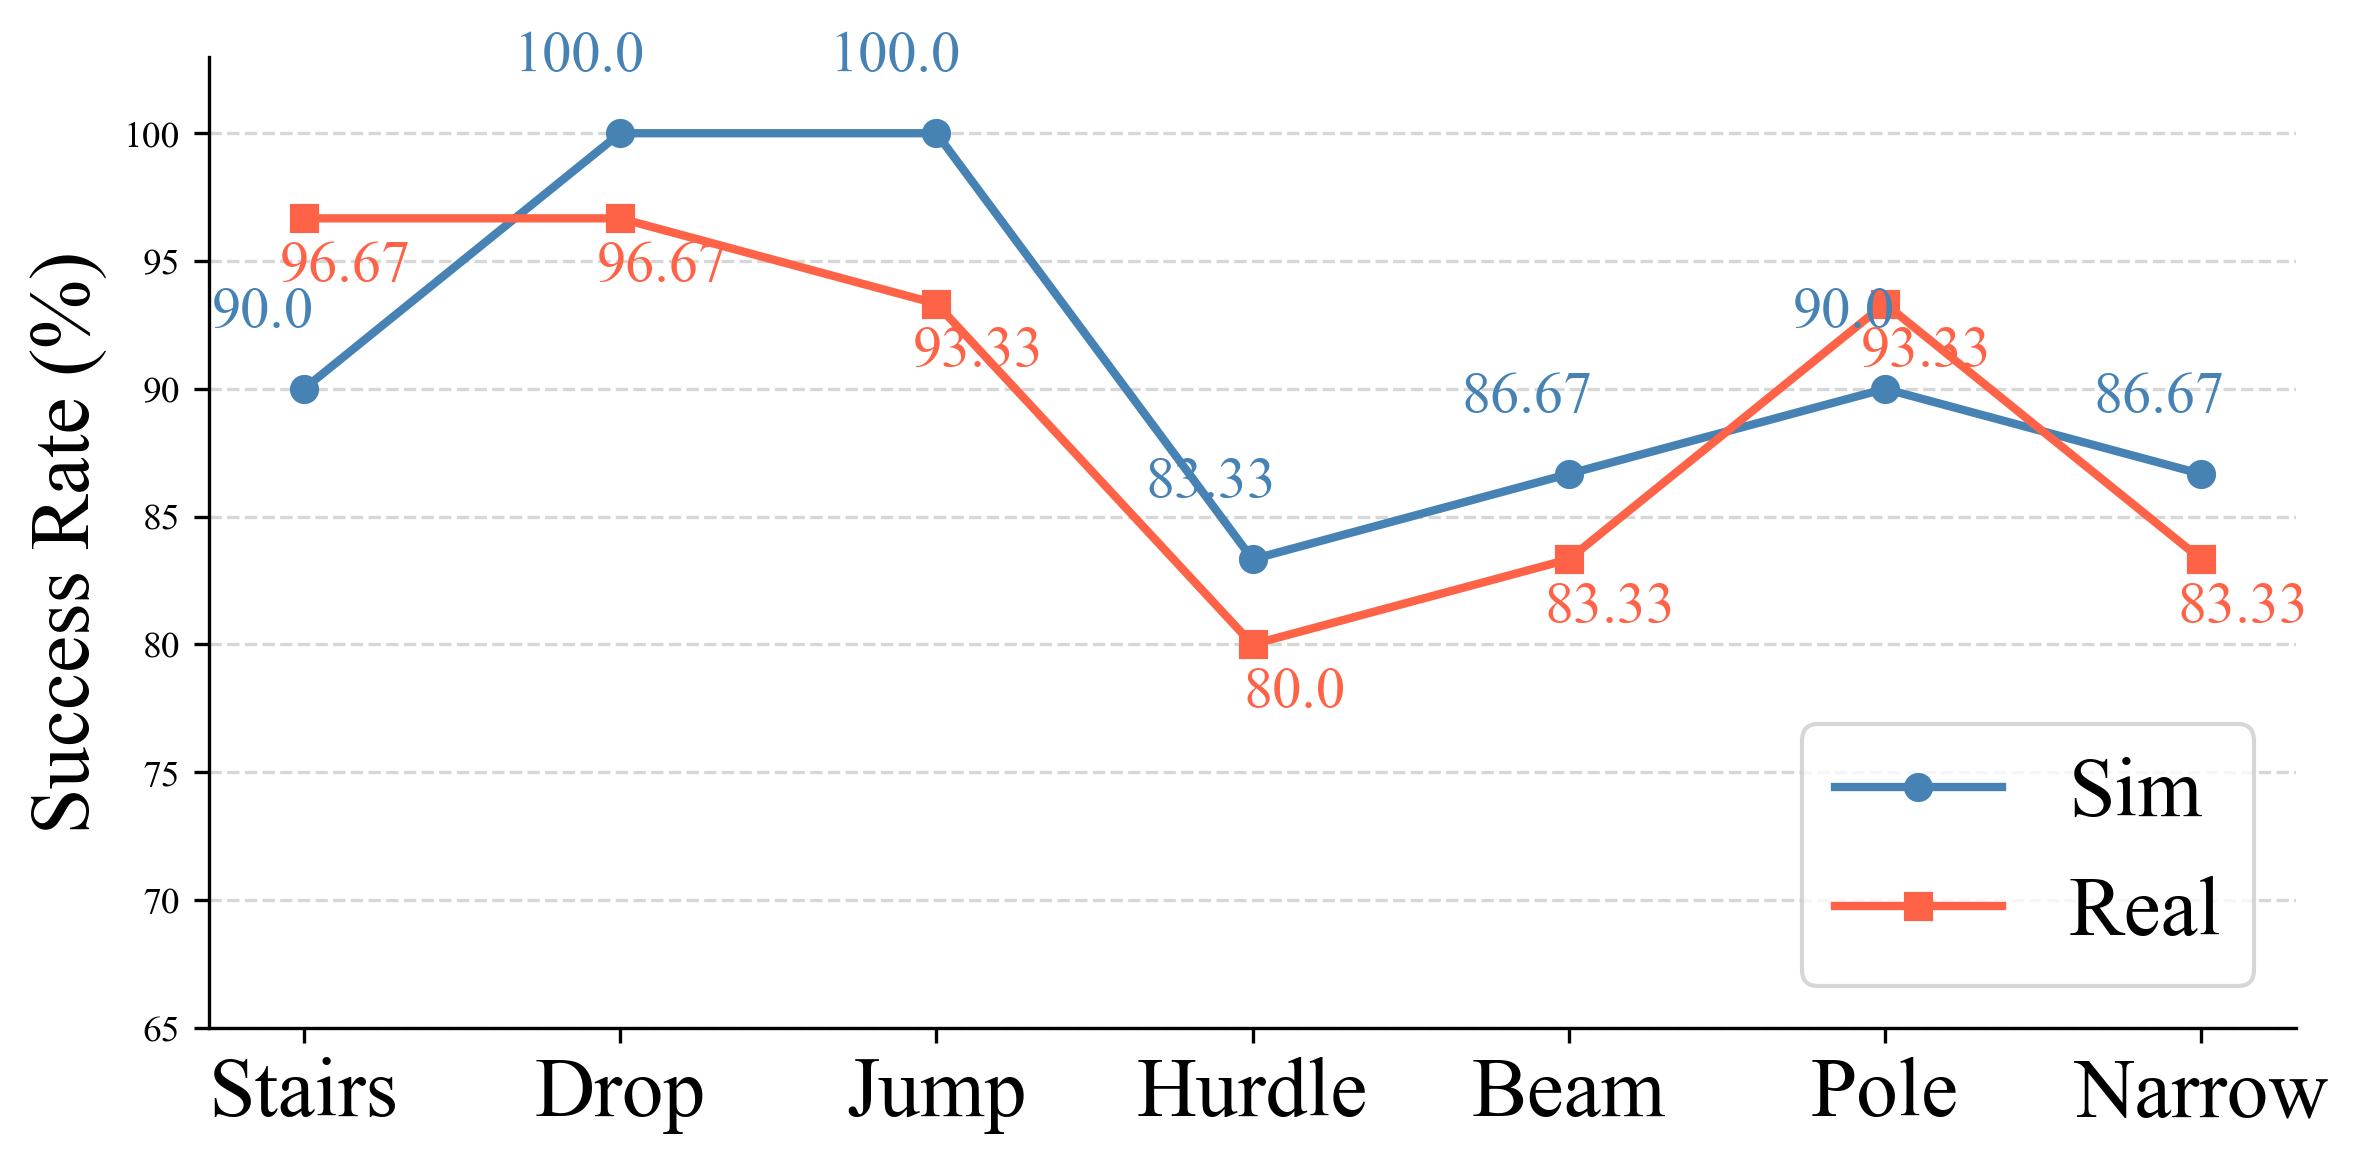
\includegraphics[width=0.9\linewidth]{figure/success_rate_sim_real.png}
    \caption{Success rates across seven terrains in simulation and real-world deployment. The real-world results for each terrain are averaged over 30 trials. }
    \label{fig:succ}
    % \vspace{-5pt}
\end{figure}

Fig.~\ref{fig:succ} presents per-terrain success rates from both simulation and physical deployment. Despite an inherent sim-to-real domain gap, the real-world success rates closely follow the trend of their counterparts in simulation, maintaining over $80\%$ success rates across all terrains. The physical robot exhibits a range of whole-body behaviors, including stair ascent and descent, stepping across drops and gaps, crouching under beams of varying height, and navigating through narrow passages and pole fields, suggesting good generality and practical applicability of the learned policy. 

% \subsection{Discussion}

% The consistent sim-to-real performance confirms that ADAPT's two design choices—the vertical distance map for compact 3D constraint encoding and the adaptive sensing radius for online horizon regulation—are more effective than heavy 3D reconstruction or multi-stage training. Well-structured inputs matter more than model complexity for agile humanoid navigation.
